\chapter{Probability}\label{chap:Probability}

\section{Basic Terminology}

\begin{definition}
    A statistical or random \vocab{experiment} (or trial) refers to a process that generates a set of observable outcomes, and can be repeated under the same set of conditions.
\end{definition}

\begin{definition}
    The \vocab{sample space} (or possibility space) $S$ of an experiment is the set of all possible outcomes of the experiment.
\end{definition}

\begin{definition}
    An \vocab{event} $E$ is a subset of $S$. The \vocab{complement} of $E$, denoted by $E'$, is the event that $E$ does not occur, i.e. $E' = S \setminus E$.
\end{definition}

\begin{definition}
    Given a subset $G \subseteq S$, the function $n(G)$ returns the \vocab{number of possible outcomes} in $G$.
\end{definition}

\section{Probability}

\begin{definition}[Classical Probability]
    If the sample space $S$ consists of a finite number of equally likely outcomes, then the probability of an event $E$ occuring (a measure of the likelihood that $E$ occurs) is denoted $\P{E}$ and is defined as \[\P{E} = \frac{n(E)}{n(S)}.\]
\end{definition}

\begin{proposition}[Range of Probabilities]
    For any event $E$, \[\P{E} \in [0, 1].\]
\end{proposition}
\begin{proof}
    Let the sample space be $S$. Since $E \subseteq S$, we have \[0 \leq n(E) \leq n(S) \implies 0 \leq \frac{n(E)}{n(S)} \leq \frac{n(S)}{n(S)} \implies 0 \leq \P{E} \leq 1.\]
\end{proof}

\begin{corollary}
    Let $A$ and $B$ be any two events. If $A \subseteq B$, then $\P{A} \leq \P{B}$.
\end{corollary}
\begin{proof}
    Identical as above.
\end{proof}

\begin{definition}
    When $\P{E} = 0$, we say that $E$ is an \vocab{impossible} event. When $\P{E} = 1$, we say that $P$ is a \vocab{sure} event.
\end{definition}

\begin{proposition}[Probability of Complement]
    For any event $E$, \[\P{E} + \P{E'} = 1.\]
\end{proposition}
\begin{proof}
    Let the sample space be $S$. By definition, $E' = S \setminus E$. Hence, \[n(E') = n(S) - n(E) \implies \frac{n(E)}{n(S)} + \frac{n(E')}{n(S)} = \frac{n(S)}{n(S)} \implies \P{E} + \P{E'} = 1.\]
\end{proof}

\begin{definition}
    Let $S$ be the sample space of a random experiment and $A$, $B$ be any two events.
    \begin{itemize}
        \item The \vocab{intersection} of $A$ and $B$, denoted by $A \cap B$, is the event that both $A$ and $B$ occur.
        \item The \vocab{union} of $A$ and $B$, denoted by $A \cup B$, is the event that at least one occurs.
    \end{itemize}
\end{definition}

\begin{proposition}[Inclusion-Exclusion Principle]
    Let $A$ and $B$ be any two events in a sample space $S$. Then \[\P{A \cup B} = \P{A} + \P{B} - \P{A \cap B}.\]
\end{proposition}
\begin{proof}
    When we take the sum of the number of outcomes in events $A$ and $B$, i.e. $n(A) + n(B)$, we will count the `overlap', i.e. $n(A \cap B)$, twice. Hence, \[n(A \cup B) = n(A) + n(B) - n(A \cap B).\] Dividing throughout by $n(S)$ yields the desired result.
\end{proof}

\begin{proposition}[Intersection of Complements]
    Let $A$ and $B$ be any two events. Then \[\P{A} = \P{A \cap B} + \P{A \cap B'}.\]
\end{proposition}
\begin{proof}
    By definition, $B' = S \setminus B$. Taking the intersection with $A$ on both sides, \[\P{A \cap B'} = \P{A \cap S} - \P{A \cap B} \implies \P{A \cap B} + \P{A \cap B'} = \P{A}.\]
\end{proof}

\begin{proposition}[``Neither Nor'']
    Let $A$ and $B$ be any two events. Then \[\P{A' \cap B'} = 1 - \P{A \cup B}.\]
\end{proposition}
\begin{proof}
    In layman terms, the above statement translates to \[\P{\text{neither $A$ nor $B$}} = 1 - \P{\text{$A$ or $B$}},\] which is clearly true.
\end{proof}

\section{Mutually Exlusive Events}

\begin{definition}
    Two events $A$ and $B$ are said to be \vocab{mutually exclusive} if they cannot occur at the same time. Mathematically, \[\P{A \cap B} = 0.\]
\end{definition}

An equivalent criterion for mutual exclusivity is \[\P{A \cup B} = \P{A} + \P{B},\] which can easily be derived from $\P{A \cap B} = 0$ via the inclusion-exclusion principle.

\section{Conditional Probability and Independent Events}

\begin{proposition}[Conditional Probability]
    The probability of an event $A$ occuring, given that another event $B$ has already occured, is given by \[\P{A}{B} = \frac{\P{A \cap B}}{\P{B}}.\]
\end{proposition}
\begin{proof}
    Since $B$ has already occured, the sample space is reduced to $B$. Hence, \[\P{A}{B} = \frac{n(A \cap B)}{n(B)}.\] Dividing the numerator and denominator by $n(S)$ completes the proof.
\end{proof}

\begin{corollary}
    The event ($A$, given $B$) is the complement of the event (not $A$, given $B$), i.e. \[\P{A}{B} + \P{A'}{B} = 1.\]
\end{corollary}
\begin{proof}
    \[\P{A}{B} + \P{A'}{B} = \frac{\P{A \cap B}}{\P{B}} + \frac{\P{A' \cap B}}{\P{B}} = \frac{\P{B}}{\P{B}} = 1.\]
\end{proof}

\begin{definition}[Independent Events]
    Let $A$ and $B$ be any two events. If either of the two occur without being affected by the other, then $A$ and $B$ are said to be \vocab{independent}. Mathematically, \[\P{A}{B} = \P{A}, \qquad \P{B}{A} = \P{B}.\]
\end{definition}

\begin{proposition}[Multiplication Law]
    $A$ and $B$ are independent events if and only if \[\P{A \cap B} = \P{A}\P{B}.\]
\end{proposition}
\begin{proof}
    Since $\P{A} = \P{A \cap B} / \P{B}$ and $\P{A}{B} = \P{A}$, \[\frac{\P{A \cap B}}{\P{B}} = \P{A} \iff \P{A \cap B} = \P{A}\P{B}.\]
\end{proof}

\begin{proposition}
    If events $A$ and $B$ are independent, then so are the following pairs of events:
    \begin{itemize}
        \item $A$ and $B'$,
        \item $A'$ and $B$,
        \item $A'$ and $B'$.
    \end{itemize}
\end{proposition}
\begin{proof}
    We only prove that $A'$ and $B$ are independent. The proofs for the other pairs are almost identical.

    Since $A$ and $B$ are independente events, we have $\P{A \cap B} = \P{A} \P{B}$. Now consider $\P{A' \cap B}$. \[\P{A' \cap B} = \P{B} - \P{A \cap B} = \P{B} - \P{A}\P{B} = \P{B} \bs{1 - \P{A}} = \P{B} \P{A'}.\] Hence, $A'$ and $B$ are independent.
\end{proof}

\section{Common Heuristics used in Solving Probability Problems}

\begin{recipe}[Table of Outcomes]
    Table of outcomes are useful as they serve as a systematic way of listing all the possible outcomes.
\end{recipe}

\begin{sample}
    Two fair dices are thrown. Find the probability that the sum of the two scores is odd and at least one of the two scores is greater than 4.
\end{sample}
\begin{sampans}
    Consider the following table of outcomes.
    \begin{center}
        \begin{tabular}{|c|c|c|c|c|c|c|}
            \hline  & 1 & 2 & 3 & 4 & 5 & 6\\\hline
            1 & 2 & 3 & 4 & 5 & 6 & \cellcolor{ForestGreen!20}7 \\ \hline
            2 & 3 & 4 & 5 & 6 & \cellcolor{ForestGreen!20}7 & 8 \\ \hline
            3 & 4 & 5 & 6 & 7 & 8 & \cellcolor{ForestGreen!20}9 \\ \hline
            4 & 5 & 6 & 7 & 8 & \cellcolor{ForestGreen!20}9 & 10 \\ \hline
            5 & 6 & \cellcolor{ForestGreen!20}7 & 8 & \cellcolor{ForestGreen!20}9 & 10 & \cellcolor{ForestGreen!20}11 \\ \hline
            6 & \cellcolor{ForestGreen!20}7 & 8 & \cellcolor{ForestGreen!20}9 & 10 & \cellcolor{ForestGreen!20}11 & 12 \\ \hline
          \end{tabular}
    \end{center}
    From the table of outcomes, the required probability is clearly $\frac{10}{36}$.
\end{sampans}

\begin{recipe}[Venn Diagrams]
    Venn diagrams are useful when we need to visualize how the events are interacting with each other.
\end{recipe}

\begin{sample}
    Let $A$ and $B$ be independent events. If $\P{A' \cap B'} = 0.4$, find the range of $\P{A \cap B}$.
\end{sample}
\begin{sampans}
    Consider the following Venn diagram.
    \begin{figure}[H]\tikzsetnextfilename{351}
        \centering
        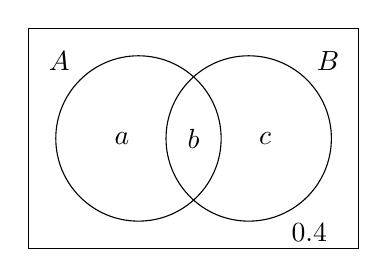
\begin{tikzpicture}[scale=0.7]
            \draw (1, 1.0) rectangle (7, 5);
            \draw (3, 3) circle[radius=1.5];
            \draw (5, 3) circle[radius=1.5];
            \node[anchor=south east] at (1.93, 4.06) {$A$};
            \node[anchor=south west] at (6.06, 4.06) {$B$};
            \node at (6.1, 1.3) {$0.4$};
            \node at (2.7, 3) {$a$};
            \node at (5.3, 3) {$c$};
            \node at (4,3) {$b$};
        \end{tikzpicture}
        \caption{}
    \end{figure}
    We see that \[a + b + c = 0.6. \tag{$\ast$}\] Further, since $A$ and $B$ are independent, we know \[\P{A \cap B} = \P{A} \P{B} \implies b = (a+b)(c+b) = (a+b)(0.6 - a).\] Expanding, we get a quadratic in $a$: \[a^2 + (b - 0.6)a + 0.4 b = 0.\] Since we want $a$ to be real, the discriminant $\D$ is non-negative. Hence, \[(b-0.6)^2 - 4(1)(0.4b) \geq 0 \implies b \leq 0.135 \quad \lor \quad b \geq 2.66.\] Since $0 \leq b \leq 1$, we reject the latter. Thus, the range of $\P{A \cap B} = b$ is $[0, 0.135]$.
\end{sampans}

\begin{recipe}[Probability Trees]
    A probability tree is a useful tool for sequential events, or events that appear in stages. The number indicated on each branch represents the conditonal probability of the event at the end node given that all the events at the previous nodes have occurred.
\end{recipe}

\begin{sample}
    Peter has a bag containing 6 black marbles and 3 white marbles. He takes out two marbles at random from the bag. Find the probability that he has taken out a black marble and a white marble.
\end{sample}
\begin{sampans}
    Consider the following propbability tree.
    \begin{figure}[H]\tikzsetnextfilename{350}
        \centering
        \begin{tikzpicture}
            \coordinate (A) at (0, 0);
            \coordinate[label=above:B] (B1) at (2, 1);
            \coordinate[label=below:W] (B2) at (2, -1);
            \coordinate[label=right:B] (C1) at (4, 1.5);
            \coordinate[label=right:W] (C2) at (4, 0.5);
            \coordinate[label=right:B] (C3) at (4, -0.5);
            \coordinate[label=right:W] (C4) at (4, -1.5);

            \draw (A) -- (B1);
            \draw (A) -- (B2);
            \draw (B1) -- (C1);
            \draw (B1) -- (C2);
            \draw (B2) -- (C3);
            \draw (B2) -- (C4);

            \node[above left] at ($(A)! 0.5 !(B1)$) {$\frac69$};
            \node[below left] at ($(A)! 0.5 !(B2)$) {$\frac39$};
            \node[above] at ($(B1)! 0.6 !(C1)$) {$\frac58$};
            \node[below] at ($(B1)! 0.6 !(C2)$) {$\frac38$};
            \node[above] at ($(B2)! 0.6 !(C3)$) {$\frac68$};
            \node[below] at ($(B2)! 0.6 !(C4)$) {$\frac28$};
        \end{tikzpicture}
        \caption{}
    \end{figure}
    The required probability is thus \[\bp{\frac69}\bp{\frac38} + \bp{\frac39}\bp{\frac68} = \frac12.\]
\end{sampans}

\begin{recipe}[Permutations and Combinations]
    Using combinatorical methods is useful when the most direct way to calculate $\P{E}$ is to find $n(E)$ and $n(S)$.
\end{recipe}

\begin{sample}
    A choir has 7 sopranos, 6 altos, 3 tenors and 4 basses. At a particular rehearsal, three members of the choir are chosen at random. Find the probability that exactly one bass is chosen.
\end{sample}
\begin{sampans}
    Note that there are a total of 20 people in the choir. Hence, the number of ways to choose three members of the choir, without restriction, is given by $\comb{20}{3}$. Meanwhile, the number of ways to choose exactly one bass is given by $\comb{4}{1} \cdot \comb{16}{2}$: first choose one bass out of the four, then choose 2 members out of the remaining 16. Thus, the required probability is \[\frac{\comb{4}{1} \cdot \comb{16}{2}}{\comb{20}3} = \frac8{19}.\]
\end{sampans}